\documentclass[border=15pt, multi, tikz]{standalone}
\usepackage{import}
\subimport{./layers/}{init}
\usetikzlibrary{positioning}
\usetikzlibrary{3d} %for including external image 

% Defining new colors for better distinction
\def\ConvColor{rgb:orange,5;red,2.5;white,4} % A warmer, more vibrant color for convolution layers
\def\ConvReluColor{rgb:orange,5;red,4;white,5} % Intensified version for convolution + ReLU layers
\def\PoolColor{rgb:blue,5;green,1;white,4} % A cooler, calming color for pooling layers
\def\DcnvColor{rgb:purple,5;blue,2.5;white,3} % Distinctive purple for deconvolution or up-sampling layers
\def\SoftmaxColor{rgb:green,5;yellow,2;white,3} % A fresh green for softmax layers, indicating output processing
\def\SumColor{rgb:cyan,5;blue,3;white,2} % Cyan for


\begin{document}
\begin{tikzpicture}
\tikzstyle{connection}=[ultra thick,every node/.style={sloped,allow upside down},draw=\edgecolor,opacity=0.7]
%%%%%%%%%%%%%%%%%%%%%%%%%%%%%%%%%%%%%%%%%%%%%%%%%%%%%%%%%%%%%%%%%%%%%%%%%%%%%%%%%%%%%%%%
%% Draw Layer Blocks
%%%%%%%%%%%%%%%%%%%%%%%%%%%%%%%%%%%%%%%%%%%%%%%%%%%%%%%%%%%%%%%%%%%%%%%%%%%%%%%%%%%%%%%%
\node[canvas is zy plane at x=0] (temp) at (-3,0,0) {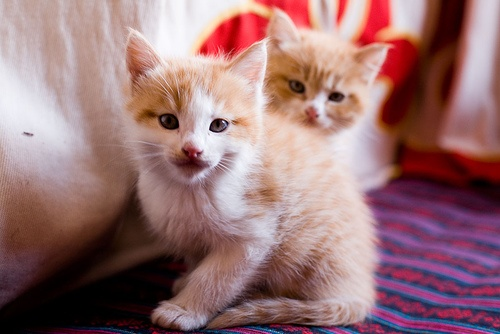
\includegraphics[width=8cm,height=8cm]{cats.jpg}};

% Conv1 + ReLU + Pool1
\pic[shift={(0,0,0)}] at (0,0,0) {RightBandedBox={name=cr1,caption=Conv1 + ReLU,%
        xlabel={{"32 filters",""}},zlabel=I,fill=\ConvColor,bandfill=\ConvReluColor,%
        height=40,width={2.5,2.5},depth=40}};
\pic[shift={(0,0,0)}] at (cr1-east) {Box={name=p1,%
        caption=Pool1, fill=\PoolColor,opacity=0.5,height=35,width=1,depth=35}};

% Conv2 + ReLU + Pool2
\pic[shift={(2,0,0)}] at (p1-east) {RightBandedBox={name=cr2,caption=Conv2 + ReLU,%
        xlabel={{"64 filters",""}},zlabel=I/2,fill=\ConvColor,bandfill=\ConvReluColor,%
        height=35,width={3.5,3.5},depth=35}};
\pic[shift={(0,0,0)}] at (cr2-east) {Box={name=p2,%
        caption=Pool2, fill=\PoolColor,opacity=0.5,height=30,width=1,depth=30}};

% Conv3 + ReLU
\pic[shift={(2,0,0)}] at (p2-east) {RightBandedBox={name=cr3,caption=Conv3 + ReLU,%
        xlabel={{"128 filters",""}},zlabel=I/4,fill=\ConvColor,bandfill=\ConvReluColor,%
        height=30,width={4.5,4.5},depth=30}};

% Flatten
\pic[shift={(1,0,0)}] at (cr3-east) {Box={name=flat,caption=Flatten,%
        fill=\PoolColor,opacity=0.5,height=23,width=1,depth=23}};

% Dense layers
\pic[shift={(1,0,0)}] at (flat-east) {RightBandedBox={name=fc,caption=Dense Layer,%
        xlabel={{"128 units",""}},zlabel=I/16,fill=\ConvColor,bandfill=\ConvReluColor,%
        height=15,width={3.5,3.5},depth=15}};

\pic[shift={(1,0,0)}] at (fc-east) {Box={name=softmax,caption=Softmax,%
        xlabel={{"",""}},fill=\SoftmaxColor,opacity=0.7,height=10,width=2,depth=10,zlabel=I/32}};

%%%%%%%%%%%%%%%%%%%%%%%%%%%%%%%%%%%%%%%%%%%%%%%%%%%%%%%%%%%%%%%%%%%%%%%%%%%%%%%%%%%%%%%%
%% Draw connections
%%%%%%%%%%%%%%%%%%%%%%%%%%%%%%%%%%%%%%%%%%%%%%%%%%%%%%%%%%%%%%%%%%%%%%%%%%%%%%%%%%%%%%%%
% Continue the connections
\draw [connection]  (p1-east)    -- node {\midarrow} (cr2-west);
\draw [connection]  (p2-east)    -- node {\midarrow} (cr3-west);
\draw [connection]  (cr3-east)   -- node {\midarrow} (flat-west);
\draw [connection]  (flat-east)  -- node {\midarrow} (fc-west);
\draw [connection]  (fc-east)    -- node {\midarrow} (softmax-west);

\end{tikzpicture}
\end{document}

